\documentclass[xetex,mathserif,serif]{beamer}
\usepackage{polyglossia}
\setdefaultlanguage[babelshorthands=true]{russian}
\usepackage{minted}
\usepackage{tabu}

\useoutertheme{infolines}

\usepackage{fontspec}
\setmainfont{FreeSans}
\newfontfamily{\russianfonttt}{FreeSans}

\tabulinesep=0.8mm

\definecolor{links}{HTML}{2A1B81}
\hypersetup{colorlinks,linkcolor=,urlcolor=links}

\title{Графический интерфейс на Java}
\author[Юрий Литвинов]{Юрий Литвинов \newline \textcolor{gray}{\small\texttt{yurii.litvinov@gmail.com}}}

\date{24.04.2019г}

\begin{document}
	
	\frame{\titlepage}
	
	\section{Введение}

	\begin{frame}
		\frametitle{Оконные библиотеки для Java}
		\begin{itemize}
			\item AWT --- очень старая, основа Swing
			\item Swing --- старая, но очень популярна
			\item SwingX --- расширение Swing
			\item JavaFX --- с Java 8 стандарт де-факто
			\item Apache Pivot --- прежде всего для веб-приложений
			\item Qt Jambi --- binding-и к Qt, требует нативных библиотек
			\item SWT --- требует нативных библиотек
		\end{itemize}
	\end{frame}

	\section{JavaFX}

	\begin{frame}
		\frametitle{JavaFX}
		\begin{center}
			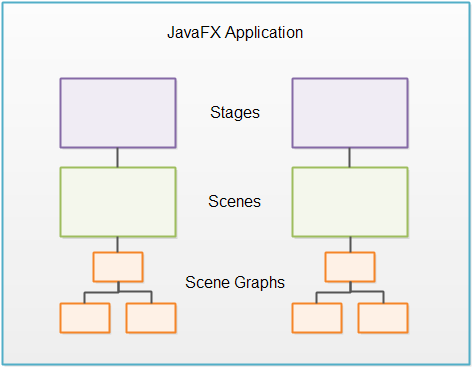
\includegraphics[width=0.6\textwidth]{javaFxOverview.png}
		\end{center}
	\end{frame}

	\begin{frame}[fragile]
		\frametitle{Минимальный пример}
		\begin{minted}{java}
import javafx.application.Application;
import javafx.stage.Stage;

public class MyFxApp extends Application {
    @Override
    public void start(Stage primaryStage) throws Exception {
        primaryStage.setTitle("My First JavaFX App");
        primaryStage.show();
    }
    
    public static void main(String[] args) {
        Application.launch(args);
    }
}
		\end{minted}
	\end{frame}

	\begin{frame}[fragile]
		\frametitle{Кнопки}
		\begin{minted}{java}
public class ButtonExperiments extends Application  {
    @Override
    public void start(Stage primaryStage) throws Exception {
        var button = new Button("Click me");

        button.setOnAction(value -> Platform.exit());

        var scene = new Scene(button, 200, 100);
        primaryStage.setScene(scene);
        primaryStage.show();
    }

    public static void main(String[] args) {
        Application.launch(args);
    }
}
		\end{minted}
	\end{frame}

	\begin{frame}
		\frametitle{Лейауты}
			\begin{tabu} {| X[1 l m] | X[1 c m] |}
				\tabucline-
				\everyrow{\tabucline-}
				BorderPane               & 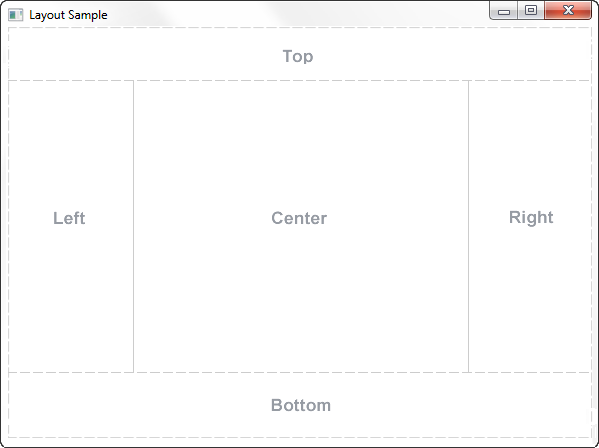
\includegraphics[height=0.2\textheight]{borderLayout.png}           \\
				HBox                     & 
\includegraphics[height=0.04\textheight]{hbox.png}                  \\
				VBox                     &                                                                     \\
				GridPane                 & 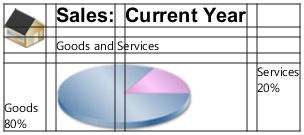
\includegraphics[height=0.1\textheight]{grid.png}                   \\
				AnchorPane               & 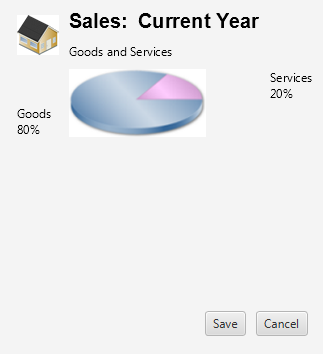
\includegraphics[height=0.2\textheight]{anchor.png}                 \\
				...                      & 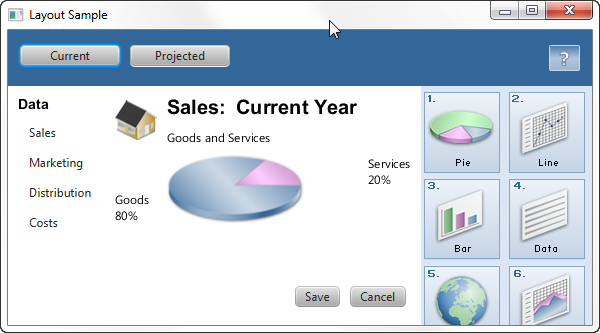
\includegraphics[height=0.1\textheight]{anchorInBorderSmall.png} \\
			\end{tabu}
	\end{frame}

	\begin{frame}[fragile]
		\frametitle{Пример, GridPane}
		\begin{scriptsize}
			\begin{minted}{java}
var button1 = new Button("Click me");
button1.setMaxSize(Double.MAX_VALUE, Double.MAX_VALUE);
button1.setOnAction(value -> Platform.exit());

var button2 = new Button("Or me");
button2.setMaxSize(Double.MAX_VALUE, Double.MAX_VALUE);
button2.setOnAction(value -> Platform.exit());

var pane = new GridPane();

var column1 = new ColumnConstraints();
column1.setPercentWidth(50);

var column2 = new ColumnConstraints();
column2.setPercentWidth(50);

var row = new RowConstraints();
row.setPercentHeight(100);
row.setFillHeight(true);

pane.getColumnConstraints().addAll(column1, column2);
pane.getRowConstraints().add(row);
			\end{minted}
		\end{scriptsize}
	\end{frame}

	\begin{frame}
		\frametitle{Геометрия GridPane}
		\begin{center}
			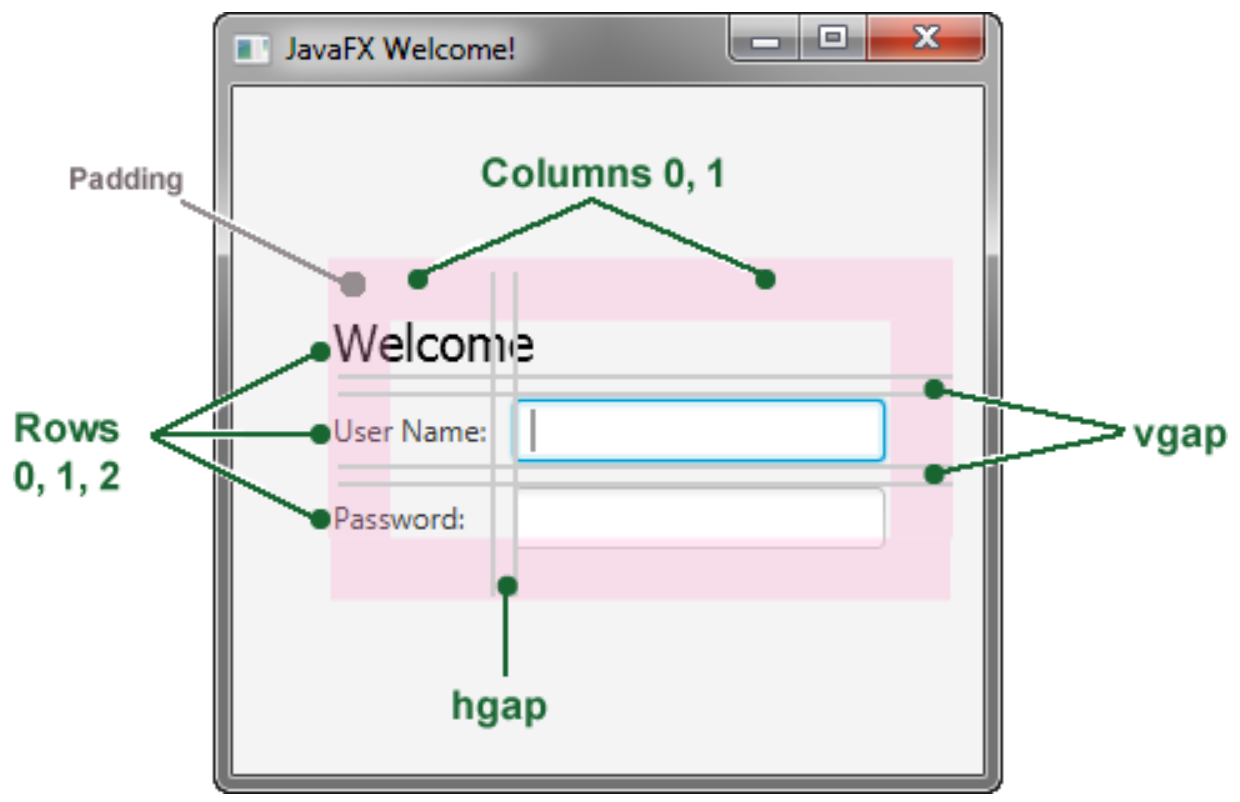
\includegraphics[width=0.7\textwidth]{gridGeometry.png}
		\end{center}
	\end{frame}

	\begin{frame}
		\frametitle{Элементы управления}
		\framesubtitle{Controls}
		\begin{center}
			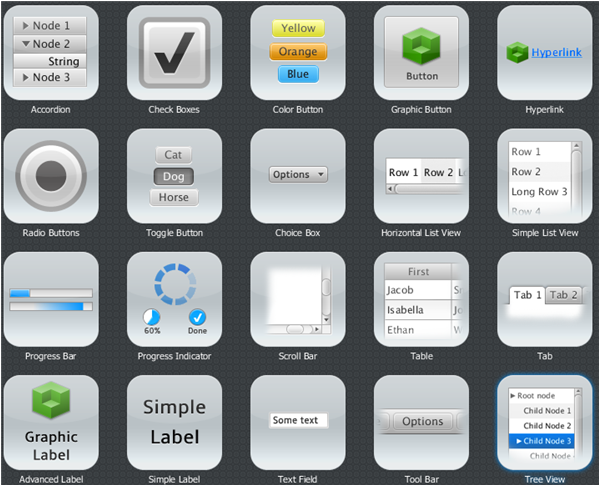
\includegraphics[width=0.7\textwidth]{javaFxControls.png}
		\end{center}
	\end{frame}

	\begin{frame}[fragile]
		\frametitle{Bindings}
		\begin{itemize}
			\item \mintinline{java}|Property<T>| --- свойство, на которое можно подписываться и которое можно автоматом менять
			\item \mintinline{java}|ObservableValue<T>|, \mintinline{java}|WritableValue<T>|
			\item Паттерн node.someProperty(), node.setSome(), node.getSome()
		\end{itemize}
		\begin{scriptsize}
			\begin{minted}{java}
public class CircleApp extends Application {
    public void start(Stage primaryStage) {
        var pane = new Pane();
        var circle = new Circle();
        circle.centerXProperty().bind(pane.widthProperty().divide(2));
        circle.centerYProperty().bind(pane.heightProperty().divide(2));
        circle.radiusProperty().bind(pane.widthProperty().divide(2).subtract(30));
        pane.getChildren().add(circle);

        var scene = new Scene(pane, 200, 200);
        primaryStage.setTitle("CircleApp");
        primaryStage.setScene(scene);
        primaryStage.show();
    }
}
			\end{minted}
		\end{scriptsize}
	\end{frame}

	\begin{frame}
		\frametitle{Canvas}
		\begin{itemize}
			\item Canvas
			\item GraphicsContext
		\end{itemize}
		\begin{center}
			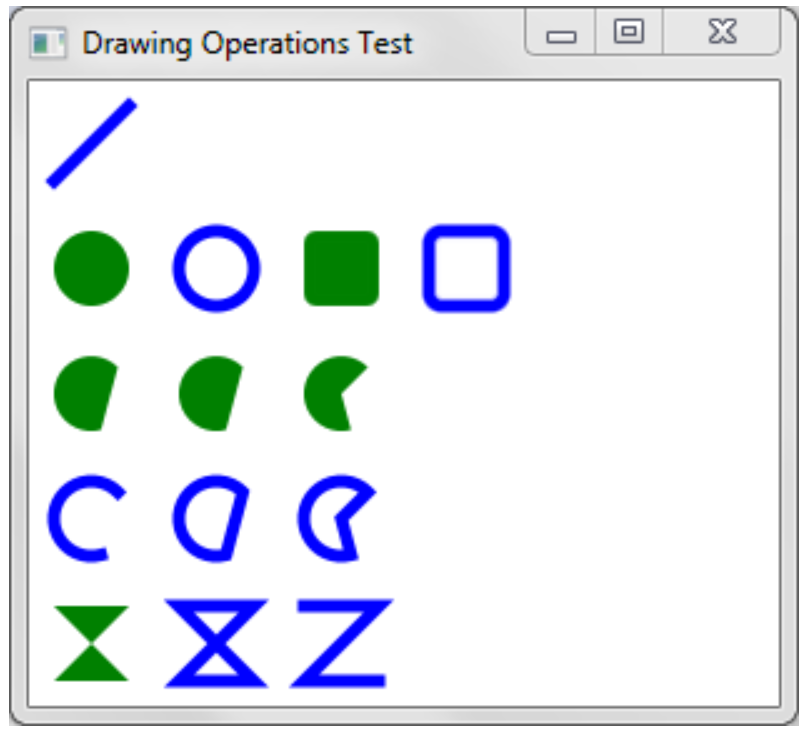
\includegraphics[width=0.4\textwidth]{canvas.png}
		\end{center}
	\end{frame}

	\begin{frame}
		\frametitle{Стили}
		\framesubtitle{CSS}
		\begin{center}
			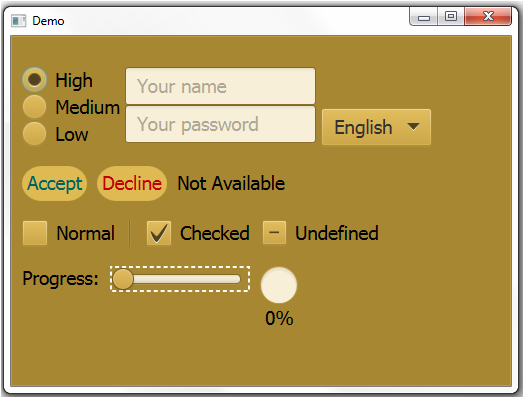
\includegraphics[width=0.6\textwidth]{styles.png}
		\end{center}
	\end{frame}

	\begin{frame}[fragile]
		\frametitle{Пример, установка стиля}
		Java:
		\begin{minted}{java}
var scene = new Scene(new Group(), 500, 400);
scene.getStylesheets().add("path/stylesheet.css");
		\end{minted}
		\vspace{1cm}
		CSS (path/stylesheet.css):
		\begin{minted}{css}
.custom-button {
    -fx-font: 16px "Serif";
    -fx-padding: 10;
    -fx-background-color: #CCFF99;
}
		\end{minted}
\end{frame}

	\begin{frame}[fragile]
		\frametitle{FXML}
		\begin{minted}{xml}
<?xml version="1.0" encoding="UTF-8"?>
<?import javafx.scene.control.*?>
<?import javafx.scene.layout.*?>
<?import javafx.scene.text.*?>
<GridPane alignment="center" hgap="10" vgap="10">
    <Text id="hello-word-text" text="Hello, world!"
            GridPane.columnIndex="0"
            GridPane.rowIndex="0" GridPane.halignment="CENTER"/>
    <Button text="Ok" GridPane.columnIndex="0"
            GridPane.rowIndex="1" GridPane.halignment="CENTER"/>
</GridPane>
		\end{minted}
\end{frame}

	\begin{frame}[fragile]
		\frametitle{FXML, в коде}
		\begin{minted}{java}
public class FXMLExample extends Application {
    @Override
    public void start(Stage stage) throws Exception {
        Parent root = FXMLLoader.load(
            new File("fxmlExample.fxml").toURI().toURL());

        stage.setTitle("FXML Welcome");
        stage.setScene(new Scene(root, 300, 275));
        stage.show();
    }

    public static void main(String[] args) {
        Application.launch(FXMLExample.class, args);
    }
}
		\end{minted}
	\end{frame}

	\begin{frame}[fragile]
		\frametitle{Сборка в gradle}
		\begin{footnotesize}
			\begin{minted}{groovy}
plugins {
    id 'java'
    id 'application'
    id 'org.openjfx.javafxplugin' version '0.0.7'
}

javafx {
    version = "11.0.2"
    modules = [ 'javafx.controls' ]
}

group 'com.example'
version '1.0-SNAPSHOT'

sourceCompatibility = 11

repositories {
    mavenCentral()
}
			\end{minted}
		\end{footnotesize}
	\end{frame}

	\section{Задание}

	\begin{frame}
		\frametitle{Задание на пару, крестики-нолики}
		Разработать приложение, позволяющие пользователю играть с самим собой в крестики-нолики. 
		\begin{itemize}
			\item На экранной форме должно быть 9 кнопок, расположенных в три столбца и три строки
			\item При первоначальном нажатии на любую из кнопок, на ней появляется знак <<Х>> 
			\item При дальнейшем нажатии на другую кнопку, на ней появляется знак <<O>>
			\item Повторное нажатие на кнопку не должно менять ее знака
		\end{itemize}
	\end{frame}

\end{document}
